
\ifdefined\ishandout
\documentclass[11pt,english,handout]{beamer}
\else
\documentclass[11pt,english]{beamer}
\fi

%\documentclass[11pt]{beamer}
\usepackage{mathptmx}
\renewcommand{\sfdefault}{lmss}
\renewcommand{\familydefault}{\sfdefault}
\usepackage[T1]{fontenc}
\usepackage[latin9]{inputenc}
\usepackage{amsmath}
\usepackage{amssymb}
\usepackage{graphicx}
\PassOptionsToPackage{normalem}{ulem}
\usepackage{ulem}
\usepackage{caption}
\captionsetup{labelformat=empty}
\usepackage{bbm}
\usepackage{upgreek}
\usepackage{graphicx}
\setbeamertemplate{section in toc}[sections numbered]
\makeatletter
\usepackage{caption} 
\usepackage{bm}
\usepackage{subfig}
\captionsetup[table]{skip=10pt}
\usepackage{pdflscape}
%%%%%%%%%%%%%%%%%%%%%%%%%%%%%% Textclass specific LaTeX commands.
% this default might be overridden by plain title style
\newcommand\makebeamertitle{\frame{\maketitle}}%
% (ERT) argument for the TOC
\AtBeginDocument{%
	\let\origtableofcontents=\tableofcontents
	\def\tableofcontents{\@ifnextchar[{\origtableofcontents}{\gobbletableofcontents}}
	\def\gobbletableofcontents#1{\origtableofcontents}
}

%%%%%%%%%%%%%%%%%%%%%%%%%%%%%% User specified LaTeX commands.
%\documentclass[presentation]{beamer}


\def\Tiny{\fontsize{7pt}{8pt}\selectfont}
\def\Normal{\fontsize{8pt}{10pt}\selectfont}

\usetheme{Madrid}
\usecolortheme{lily}
%\setbeamercovered{transparent}
\useinnertheme{rounded}


\setbeamertemplate{footline}{\hfill\Normal{\insertframenumber/\inserttotalframenumber}}
%\setbeamertemplate{footline}{}

\setbeamertemplate{navigation symbols}{}

\newenvironment{changemargin}[2]{%
	\begin{list}{}{%
			\setlength{\topsep}{0pt}%
			\setlength{\leftmargin}{#1}%
			\setlength{\rightmargin}{#2}%
			\setlength{\listparindent}{\parindent}%
			\setlength{\itemindent}{\parindent}%
			\setlength{\parsep}{\parskip}% 
		}%
		\item[]}{\end{list}}

\setbeamertemplate{footline}{\hfill\insertframenumber/\inserttotalframenumber}
\setbeamertemplate{navigation symbols}{}

%\usepackage{times}  % fonts are up to you
\usepackage{graphicx}
%\usepackage{graphics}
\usepackage{epsfig}
\usepackage{bm}
\usepackage{epsf}
\usepackage{float}
\usepackage[final]{pdfpages}
\usepackage{multirow}
\usepackage{colortbl}
\usepackage{xkeyval}
%\usepackage{sgame}
%\usepackage{pst-node}
\usepackage{listings}
\usepackage{ifthen}
%\usepackage{hyperref}
\usepackage{tikz}

%\usepackage{times}  % fonts are up to you
%\usepackage{graphicx}
%\usepackage{graphics}
\usepackage{epsfig,bm,epsf,float}
\usepackage[final]{pdfpages}
\usepackage{xcolor,multirow,colortbl}
\usepackage{xkeyval}
\usepackage{verbatim}
%\usepackage{sgame}
%\usepackage{pst-node}
\usepackage{listings}
%\usepackage{handoutWithNotes}
%\pgfpagesuselayout{3 on 1 with notes}[letterpaper,border shrink=5mm]
%\pgfpagesuselayout{2 on 1 with notes landscape}[letterpaper,border shrink=5mm]
\usepackage{setspace}
\usepackage{ragged2e}
\usepackage{pdfpages}
\setbeamersize{text margin left=1em,text margin right=1em} % CambridgeUS spacing if you use default instead


%\pdfmapfile{+sansmathaccent.map}

% Table formatting
\usepackage{booktabs}


% Decimal align
\usepackage{dcolumn}
\newcolumntype{d}[0]{D{.}{.}{5}}


\global\long\def\expec#1{\mathbb{E}\left[#1\right]}
\global\long\def\var#1{\mathrm{Var}\left[#1\right]}
\global\long\def\cov#1{\mathrm{Cov}\left[#1\right]}
\global\long\def\prob#1{\mathrm{Prob}\left[#1\right]}
\global\long\def\one{\mathbf{1}}
\global\long\def\diag{\operatorname{diag}}
\global\long\def\expe#1#2{\mathbb{E}_{#1}\left[#2\right]}
\DeclareMathOperator*{\plim}{\text{plim}}

%\usefonttheme[onlymath]{serif}

\usepackage{appendixnumberbeamer}
\renewcommand{\thefootnote}{}

\setbeamertemplate{footline}
{
	\leavevmode%
	%   \hbox{%
	%      \begin{beamercolorbox}[wd=\paperwidth,ht=2.25ex,dp=1ex,right]{date in head/foot}%
	%\usebeamerfont{date in head/foot}\insertshortdate{}\hspace*{2em}%
	\hfill
	%turning the next line into a comment, erases the frame numbers
	\insertframenumber{}\hspace*{2ex}\vspace{1ex}
	
	%    \end{beamercolorbox}}%
}

\definecolor{blue}{RGB}{0, 0, 210}
\definecolor{red}{RGB}{170, 0, 0}

\makeatother

\usepackage[english]{babel}

\usepackage{tikz}
\newcommand*\circled[1]{\tikz[baseline=(char.base)]{             \node[circle,ball color=structure.fg, shade,   color=white,inner sep=1.2pt] (char) {\tiny #1};}} 

\makeatletter
\let\save@measuring@true\measuring@true
\def\measuring@true{%
	\save@measuring@true
	\def\beamer@sortzero##1{\beamer@ifnextcharospec{\beamer@sortzeroread{##1}}{}}%
	\def\beamer@sortzeroread##1<##2>{}%
	\def\beamer@finalnospec{}%
}
\makeatother



\setbeamersize{text margin left= .8em,text margin right=1em} 
\newenvironment{wideitemize}{\itemize\addtolength{\itemsep}{10pt}}{\enditemize}
\newenvironment{wideitemizeshort}{\itemize}{\enditemize}

\newcommand{\indep}{\perp\!\!\!\!\perp} 


\DeclareMathOperator*{\argmax}{arg\,max}
\DeclareMathOperator*{\argmin}{arg\,min}

\begin{document}
	
	%% Title slide
	\begin{frame}[noframenumbering]{}
		\vspace{0.5cm}
		\title[]{Chapter 9: Bonus content --- Additional applications}
		\author{Jonathan Roth}
		\date{Mathematical Econometrics I \\ Brown University\\Fall 2023} 
		\titlepage {\small{}\ }\thispagestyle{empty} \vspace{-30pt}
		
	\end{frame}


	\begin{frame}{Overview}
		\begin{wideitemize}
			\item
			If we've reached these slides, it means I talked slightly faster than planned this semester --- so it's time for some bonus content!
			
			\item
			I thought it would be useful to walk through a few different recent applications of the tools we learned in the course
			
			\item
			Focus will be on more recent and more diverse set of authors than earlier (not just papers by Angrist and/or Krueger!)
		\end{wideitemize}
	\end{frame}	


	\begin{frame}{Juvenile incarceration}
		\begin{wideitemize}
			\item
			The US incarcerates more people than any country in the world (about 2M people)
			
			\item
			In addition to adult incarceration, a substantial number of juveniles (people under 18) are incarcerated as well (about 70K)
			
			\item
			Anna Aizer (Brown professor!) and Joseph Doyle (2015) studied the impacts of juvenile incarceration
			
			\item
			In particular, they ask how being incarcerated as a juvenile (a) impacts future criminal activity, (b) impacts completion of education
			
		\end{wideitemize}
	\end{frame}

\begin{frame}{How do you think juvenile incarceration would impact future crime and education?}
		\begin{wideitemize}	
			\pause
			\item
			Advocates for incarceration would argue that juvenile incarceration (typically pretty short) may help prevent youths on a `downward spiral' and have a rehabilitative effect. May reduce future crime and increase education completion
			
			\item
			Critics of incarceration argue that juvenile incarcertation may be disruptive to youths and limit their possible employment outcomes $\rightarrow$ less education, more crime as adults	
		\end{wideitemize}
		
\end{frame}

\begin{frame}{Identifying causal effects}

\begin{wideitemize}
	\item
	Hopefully by this point in the course it's clear why we can't just compare youths who are incarcerated to those who aren't. Why not? \pause{} Confounding variables!
	
	\item
	Do you have any ideas about how we might get a more compelling causal answer to this question? 
	
	\pause
	\item
	Aizer and Doyle exploit the fact that in Chicago, which judge you are assigned to is effectively as good as random. They then use judge leniency as an instrumental variable
	
	\pause
	\item
	In particular, juvenile defendants are assigned to a ``calendar'' based on their neighborhood and crime type. Multiple judges are assigned to each ``calendar.'' Which judge you get on the calendar is based on idiosyncratic factors (judges essentially alternate cases).
\end{wideitemize}

\end{frame}

\begin{frame}{The judge instrument}
	\begin{wideitemize}
		\item
		Aizer and Doyle use the leniency of the judge you are assigned to as an instrumental variable.
		
		\item
		Leniency is measured as the fraction of defendants that saw that judge who were incarcerated (excluding the current defendant to avoid overfitting)
		
		\pause
		\item
		Let $Y_i$ be a defendant outcome -- e.g. do they commit a crime as an adult; do they finish HS
		
		\item
		Let $D_i$ be whether a defendant was incarcerated as a juvenile
		
		\item
		Define $Z_i$ to be the average of value of $D$ among other defendants with same judge as $i$. 
	\end{wideitemize}
\end{frame}


\begin{frame}{Evaluating the assumptions}
	\begin{wideitemize}
		\item
		\textbf{Relevance}:\pause{} defendants assigned to a stricter judge need to be more likely to be incarcerated. \pause{} Seems reasonable
		
		\item
		\textbf{Independence}:\pause{} Which judge you are assigned to needs to be independent of other determinants of adult crime and other determinants of incarceration (e.g. crime type, lawyer quality) \pause{}
			\begin{wideitemize}
				\item
				Conditional on the ``calendar'', this seems reasonable based on the institutional structure
			\end{wideitemize}
		
		\item
		\textbf{Exclusion}: \pause the stringency of the judge that you get affects future outcomes only through whether you are incarcerated.
			\begin{itemize}
				\item 
				Reasonable if judge only determines whether you're incarcerated
				
				\item
				We might worry that judges determine other things --- sentence length, probation terms, etc.
			\end{itemize}
		
		\item
		\textbf{Monotonicity}:\pause{} everyone incarcerated with a lenient judge would also be incarcerated with a stricter judge \pause
			\begin{itemize}
				\item
				Could be violated if, e.g., judge who is strict on violent crime is lenient on drug crime 
			\end{itemize}
	\end{wideitemize}
\end{frame}

\begin{frame}{Covariate balance}
	\begin{center}
	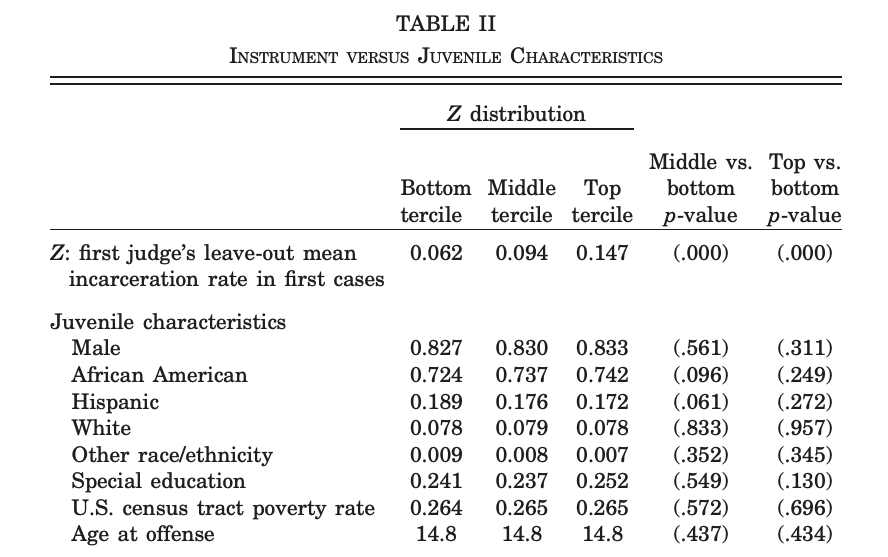
\includegraphics[width = 0.7 \linewidth]{balance}
	\end{center}
Judge leniency is not correlated with defendant characteristics
\end{frame}

\begin{frame}{Specification}
	\begin{wideitemize}
		\item
		\textbf{First stage:} regress incarceration on judge strictness, controlling for ``calendar'' and defendant characteristics
		$$D_{i} =  \pi_1 Z_i + \pi_2' X_i + \delta_{c(i)} + v_i ,$$
		
		\noindent where $X_i$ is a vector of defendant characteristics, and $\delta_{c(i)}$ is a ``calendar'' fixed effect.
		

	\end{wideitemize}
\end{frame}

\begin{frame}{First stage results}
	\begin{center}
		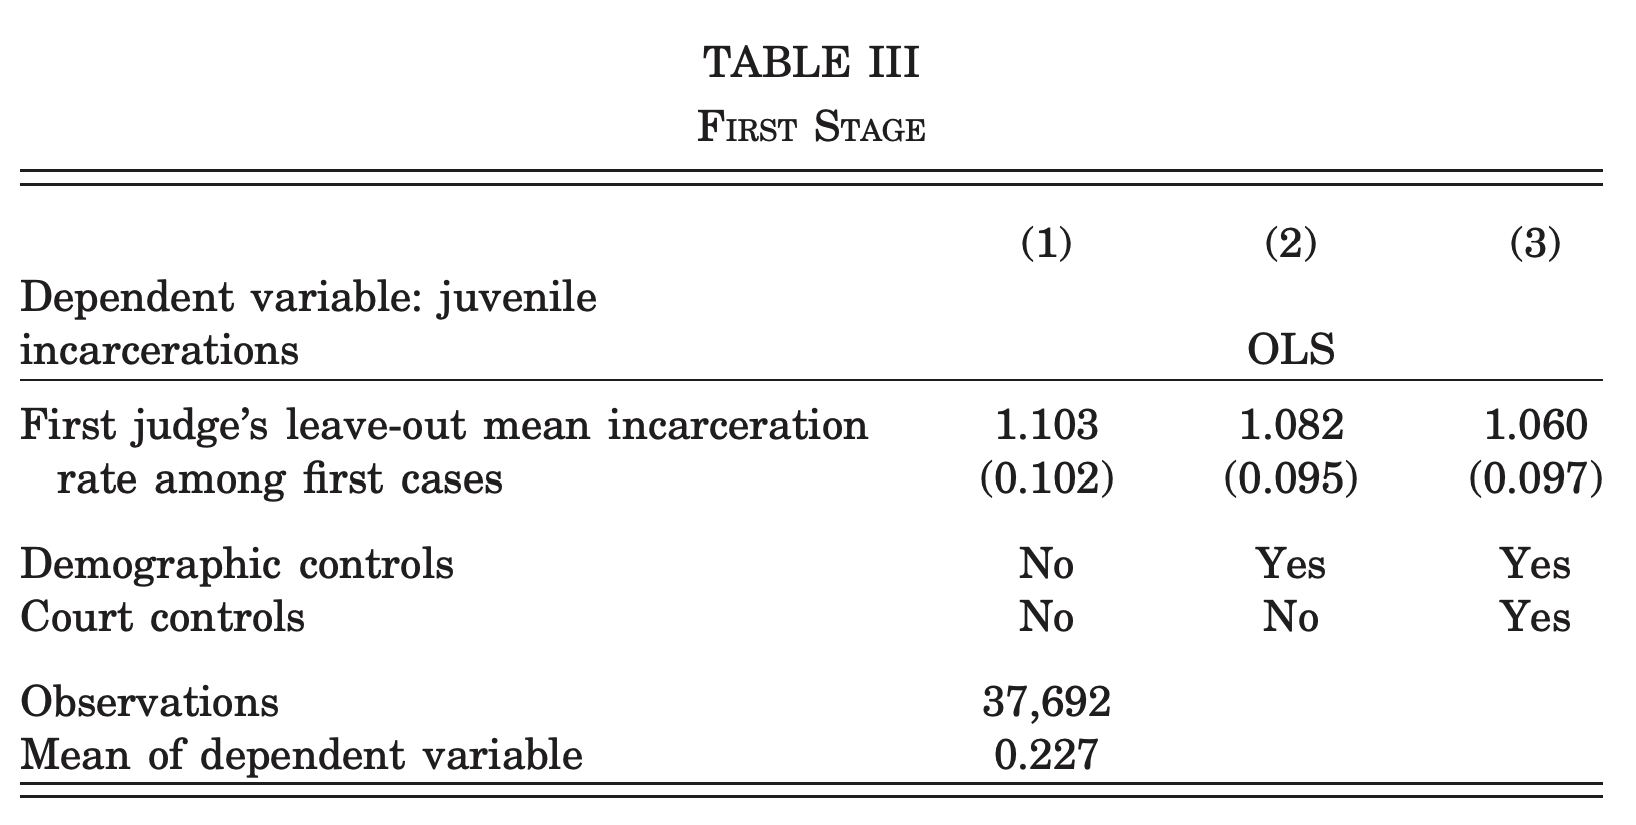
\includegraphics[width=0.7 \linewidth]{first-stage}
	\end{center}

\pause 
First stage is statistically indistinguishable from 1 $\rightarrow$ a 1 percentage point stricter judge means a 1 percentage point higher chance of incarceration (intuitive!)
\end{frame}

\begin{frame}{Specification}
	\begin{wideitemize}
		\item
		\textbf{First stage:} regress incarceration on judge strictness, controlling for ``calendar'' and defendant characteristics
		$$D_{i} =  \pi_1 Z_i + \pi_2' X_i + \delta_{c(i)} + v_i ,$$
		
		\noindent where $X_i$ is a vector of defendant characteristics, and $\delta_{c(i)}$ is a ``calendar'' fixed effect.

\pause

	\item
	\textbf{Second stage:} regress outcome of interest (HS grad, future crime) on predictions from the first-stage $\hat{D}$
	
	$$ Y_{i} = \beta_0 + \beta_1 \hat{D}_i + \beta_2'X_i + \beta_{c(i)}+ \epsilon_i $$		
		
	\end{wideitemize}
\end{frame}


\begin{frame}
	\begin{center}
		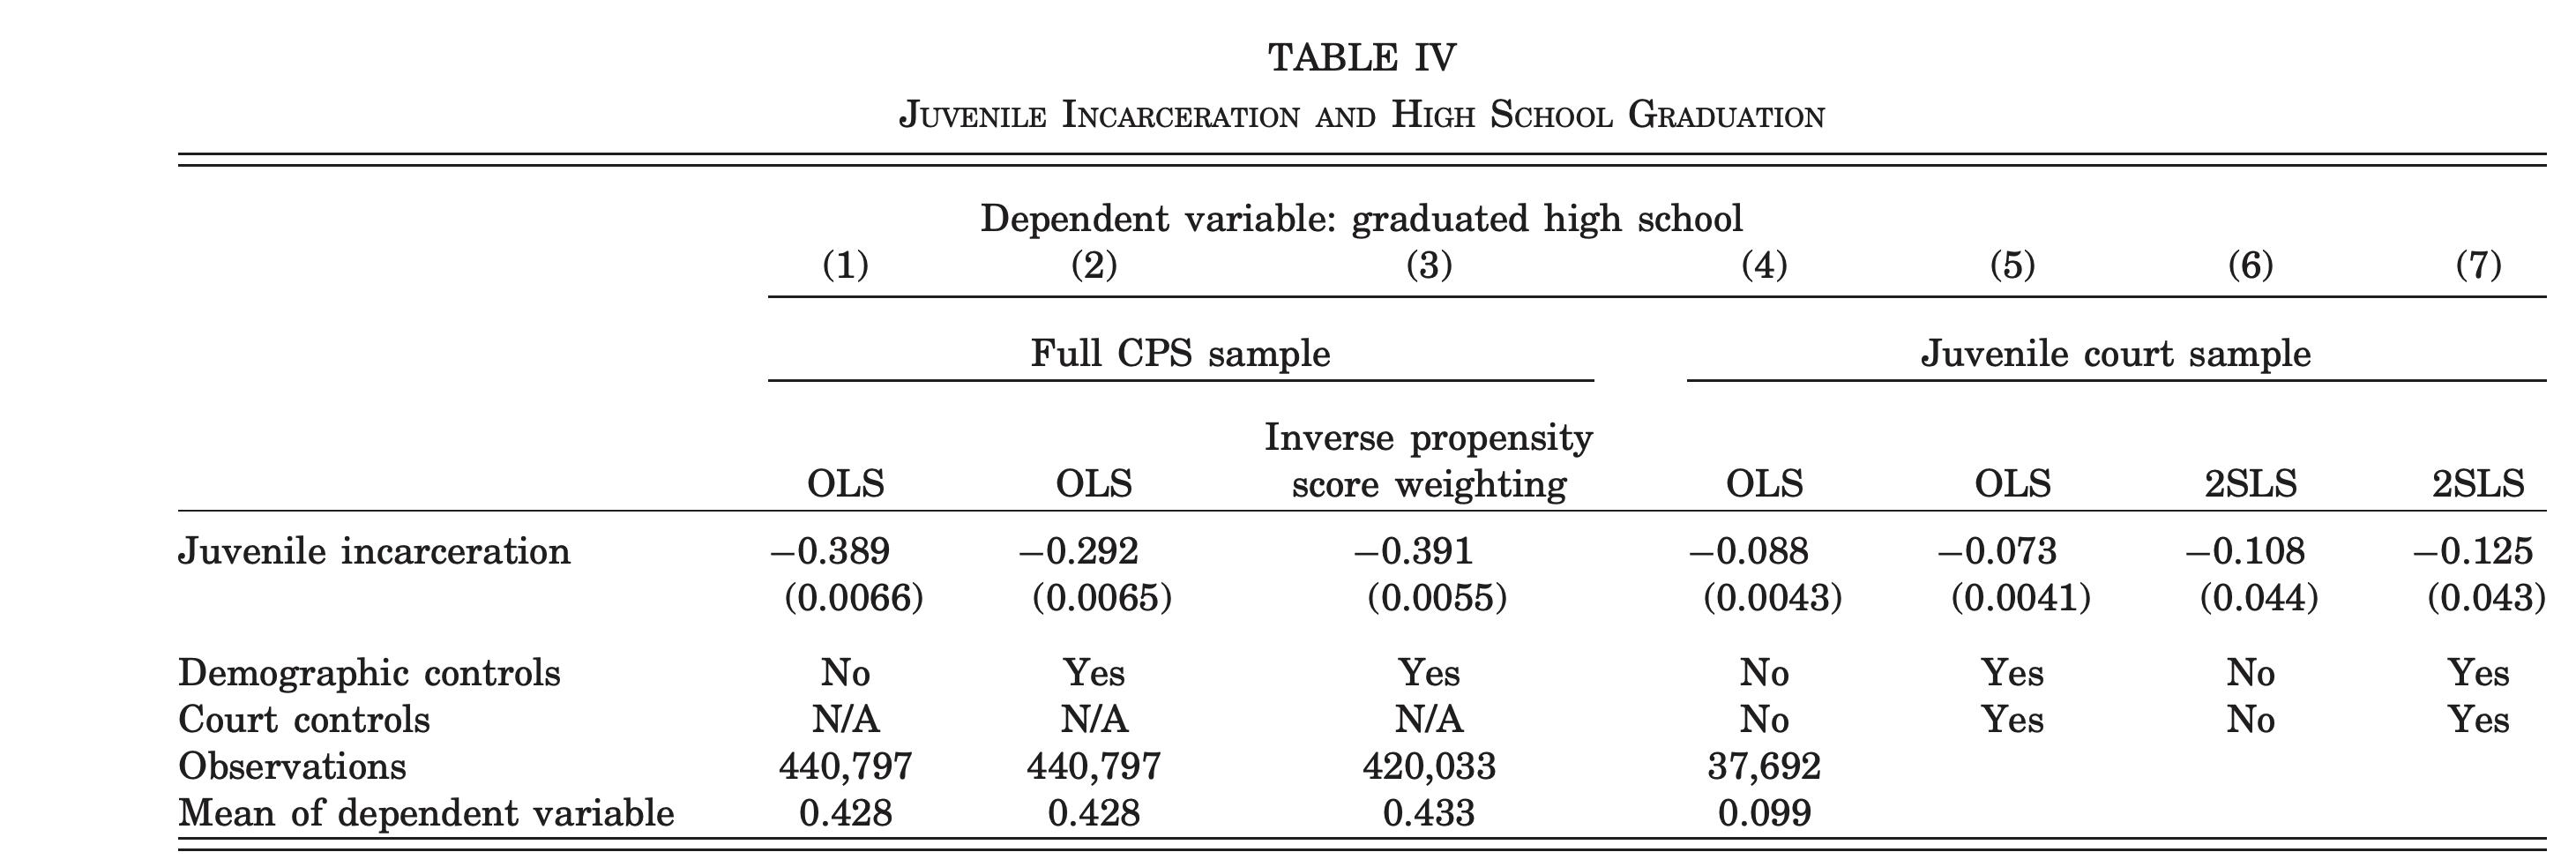
\includegraphics[width = 0.95\linewidth]{iv-graduation}
	\end{center}
\end{frame}

\begin{frame}
	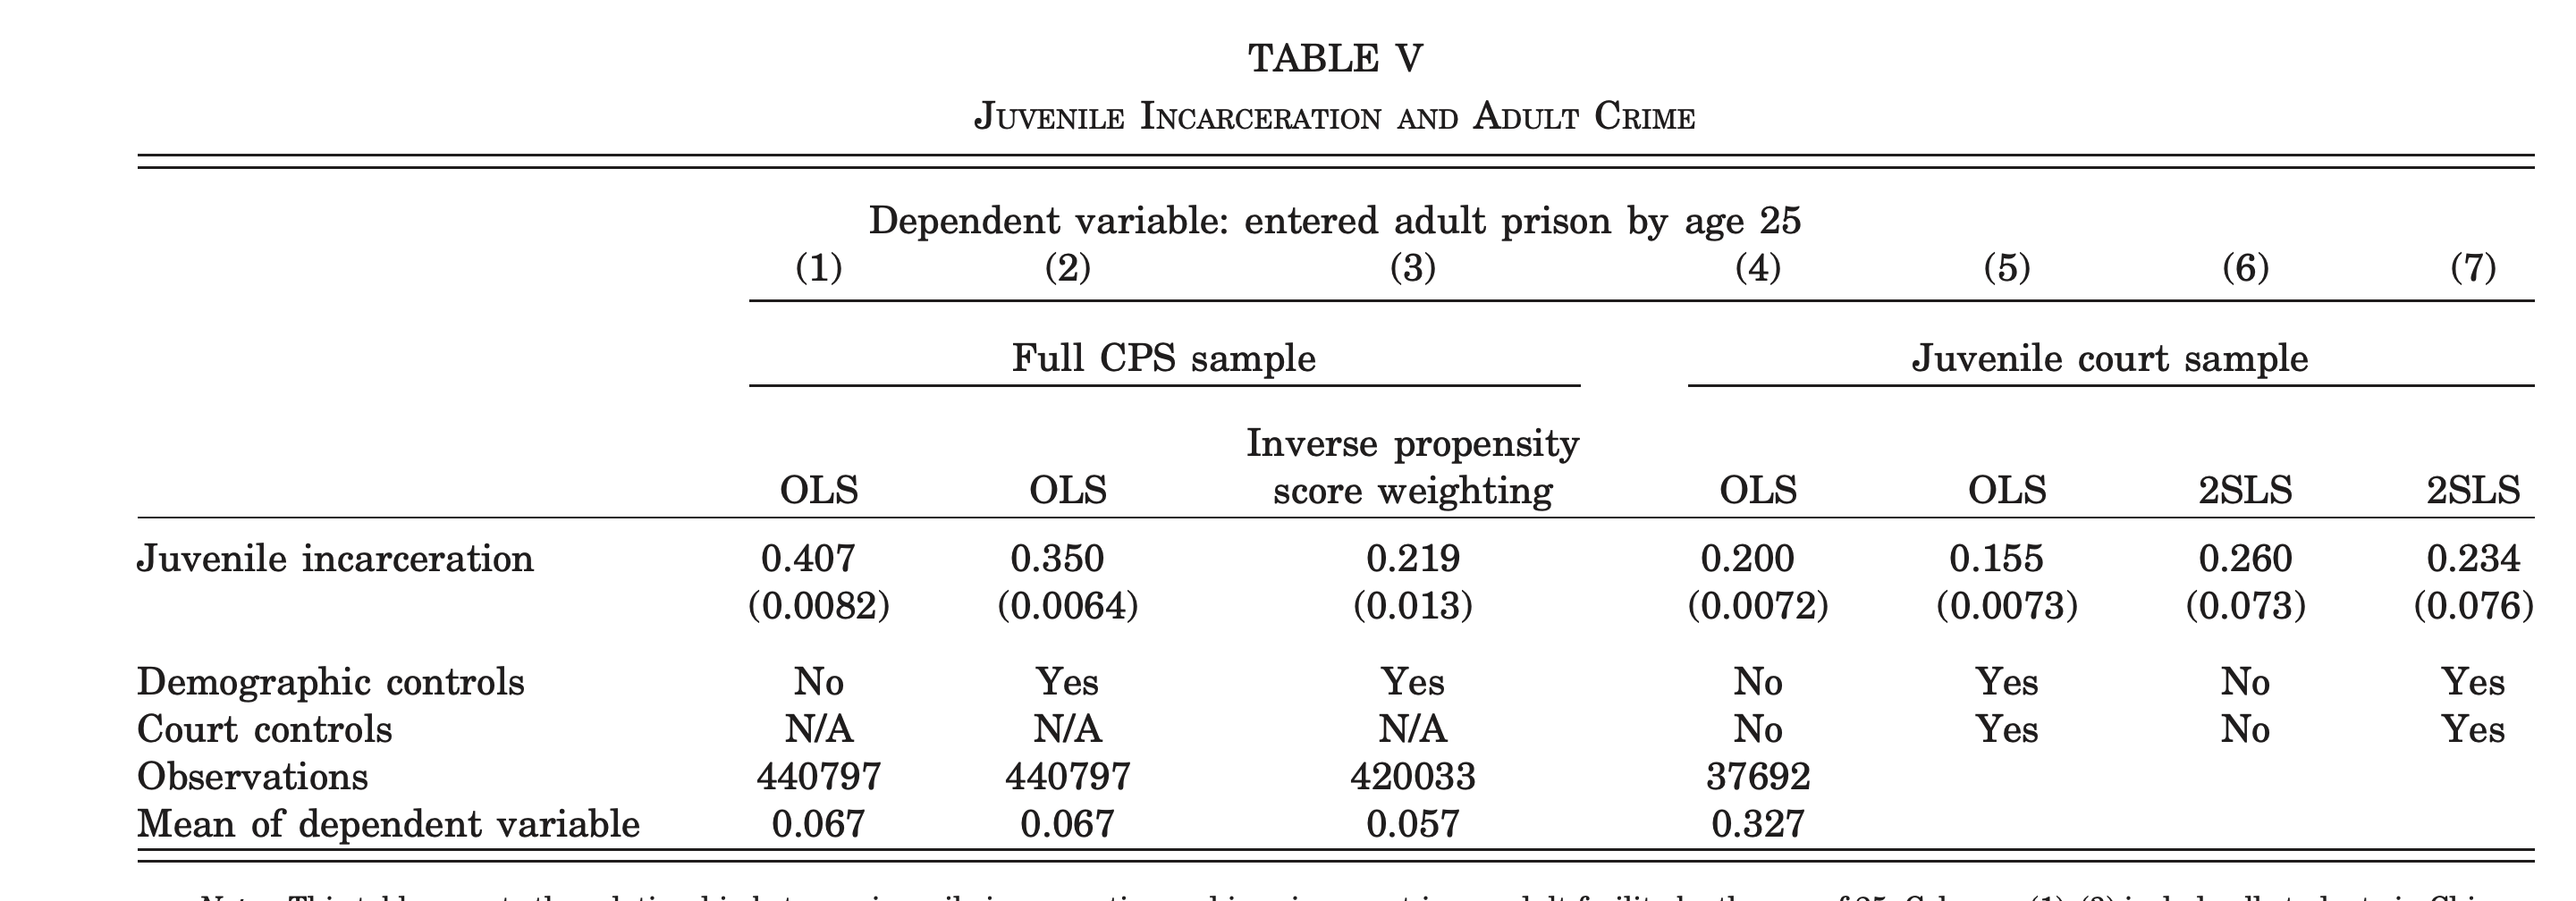
\includegraphics[width = 0.95 \linewidth]{iv-crime}
\end{frame}

\begin{frame}{Who is this a treatment effect for? }

\pause
\begin{wideitemize}
	\item
	Compliers! People who would be incarcerated only if they got a strict judge but not a lenient one
	\pause
	\item
	So this doesn't tell us that we shouldn't incarcerate anyone (maybe it's good for always takers?)
	
	\item
	But on the margin, having the strict judges rule like the lenient ones appears like it would increase HS graduation and reduce adult crime
	
	\pause
	\item
	Note, though, that this calculation does not consider the deterrence effects --- i.e., maybe people commit fewer crimes because they are worried about going to juvie
\end{wideitemize}
\end{frame}

\begin{frame}{Does incarceration always cause crime?}
\pause
\begin{wideitemize}
	\item
	Bhuller et al (2020) use a similar IV using judge stringency in Norway
	
	\item
	This study looks at adults accused of crimes in Norway
	
	\item
	In Norway, it is mandated by law that judges be randomly assigned to defendants
\end{wideitemize}

\end{frame}

\begin{frame}
	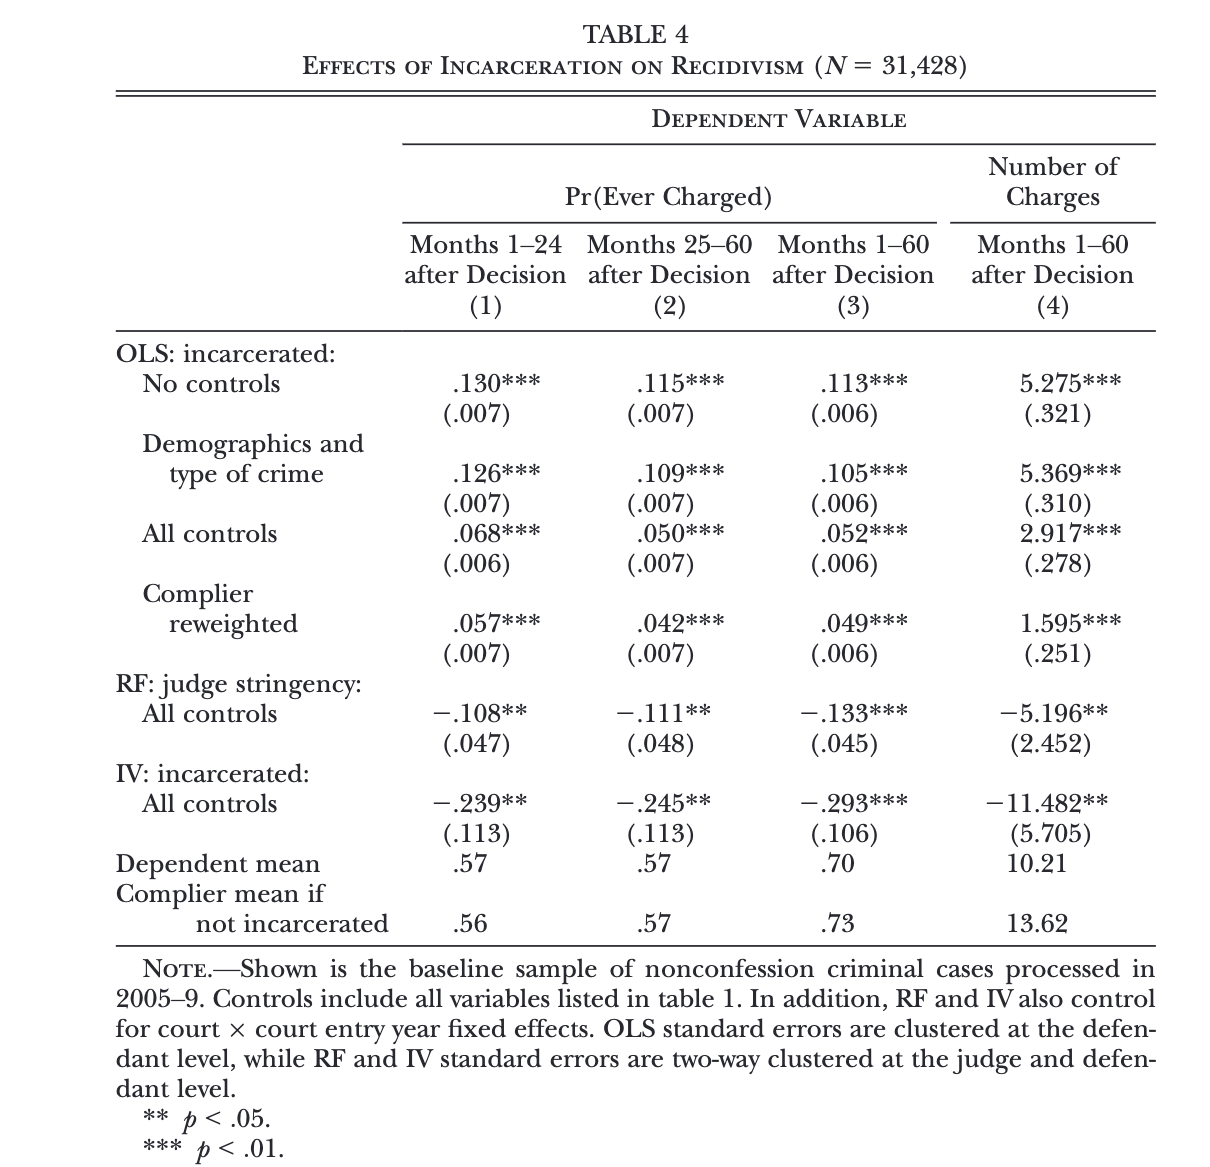
\includegraphics[width = 0.9 \linewidth]{norway-iv}
\end{frame}

\begin{frame}{Interpreting these results}
	\pause
	\begin{wideitemize}
		\item
		One initial thought might be that the reduction in recidivism is the result of incapication --- you can't commit a new crime if you're in jail
		
		\pause
		\item
		But 90\% of people incarcerated serve less than 1 year. And the effects persist for 25-60 months
		
		\pause
		\item
		Clearly, the prisons are doing something to prevent crime even after people leave
	\end{wideitemize}
\end{frame}

\begin{frame}{What do prisons in Norway do?}
	\begin{center}
		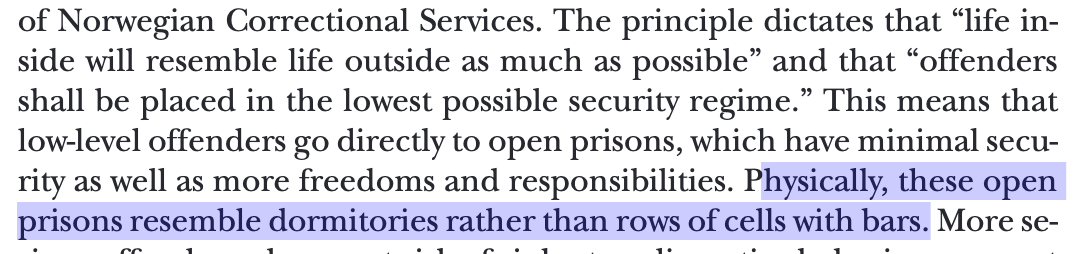
\includegraphics[width = 0.9\linewidth]{description-prison} \pause \bigskip 
		
		
		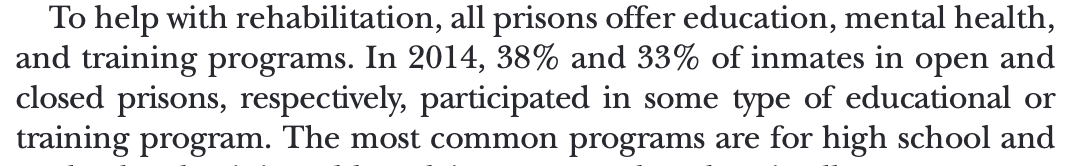
\includegraphics[width = 0.9\linewidth]{description-prison-2}
	\end{center}
\end{frame}

\begin{frame}
	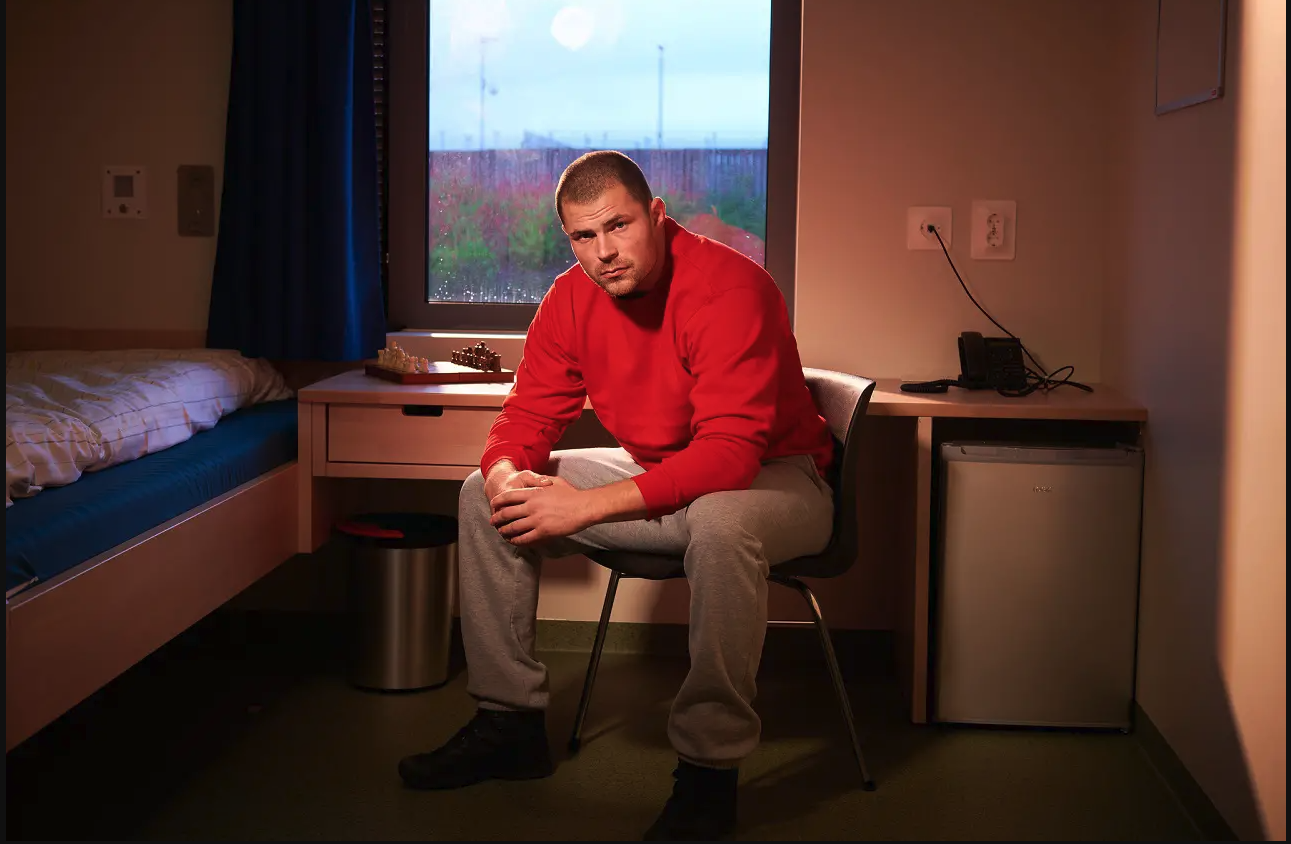
\includegraphics[width = 0.9 \linewidth]{prison-pic}
\end{frame}


\begin{frame}
	\centering
	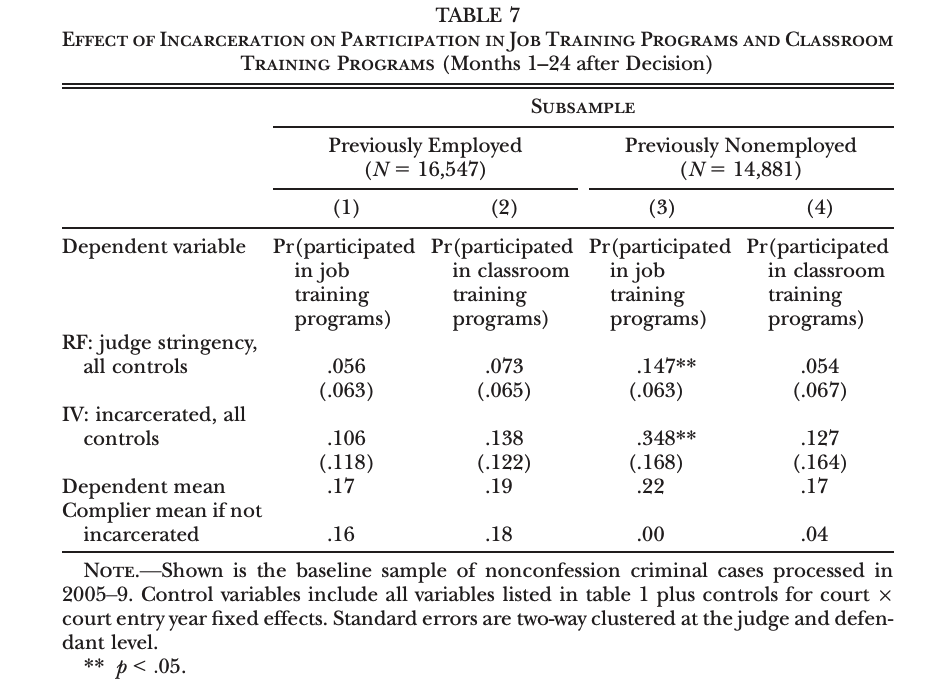
\includegraphics[width = 0.9\linewidth]{job-training}
\end{frame}

\begin{frame}
	\centering
	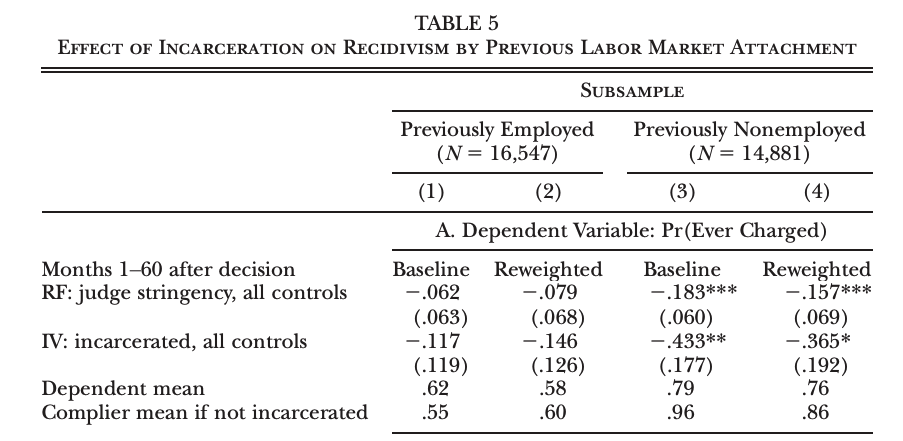
\includegraphics[width = 0.9\linewidth]{incarceration-by-attachment}
\end{frame}

\begin{frame}{To summarize}
	\begin{wideitemize}
		\item
		Prisons in Norway (in contrast to US) focus heavily on rehabilitiation and training
		
		\item
		This appears to have a positive effect on labor market outcomes for those who were not employed at baseline
		
		\item
		For those who were employed at baseline, the disruption effect may dominate the effect of additional training
	\end{wideitemize}
\end{frame}

\begin{frame}{Examiner designs}
	\begin{wideitemize}
		\item
		Similar research designs have been used in other contexts where there is an ``examiner'' who reviews a case and makes a decision of interest	
		
		\item
		Here are a few other examples
	\end{wideitemize}
\end{frame}

\begin{frame}
	\centering
	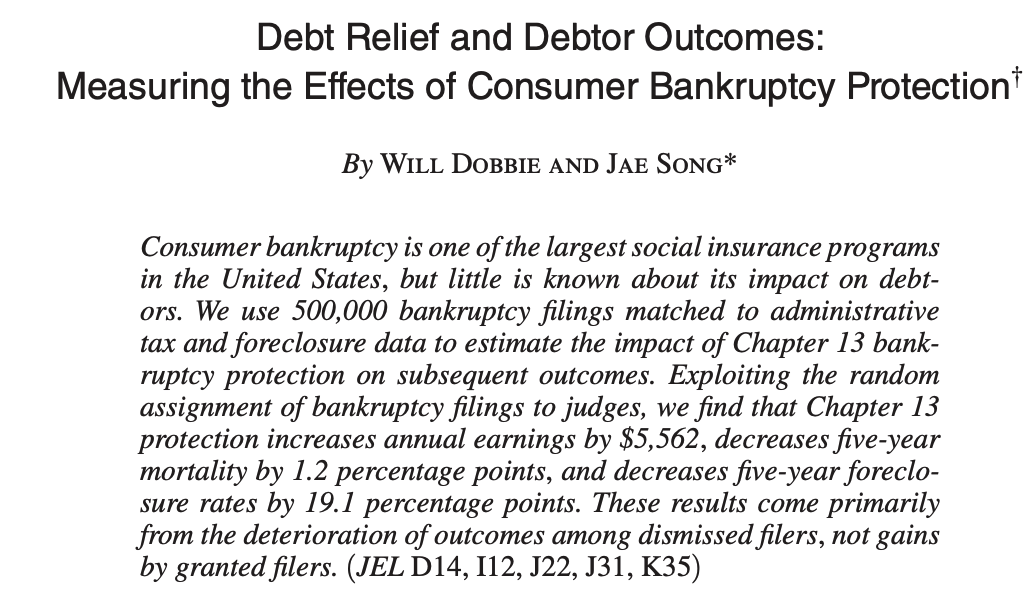
\includegraphics[width = 0.9 \linewidth]{bankruptcy-iv}
\end{frame}


\begin{frame}
	\centering
	
\includegraphics[width = 0.9 \linewidth]{foster-care-1}
	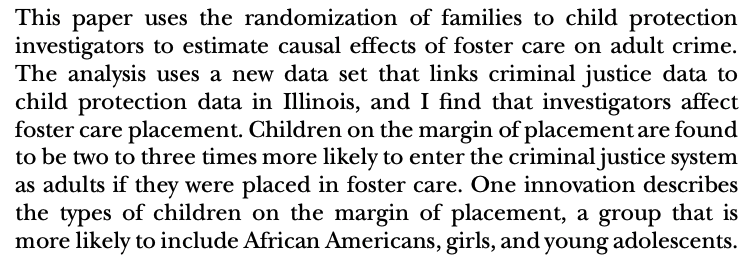
\includegraphics[width = 0.9 \linewidth]{foster-care-2}
\end{frame}

\begin{frame}
	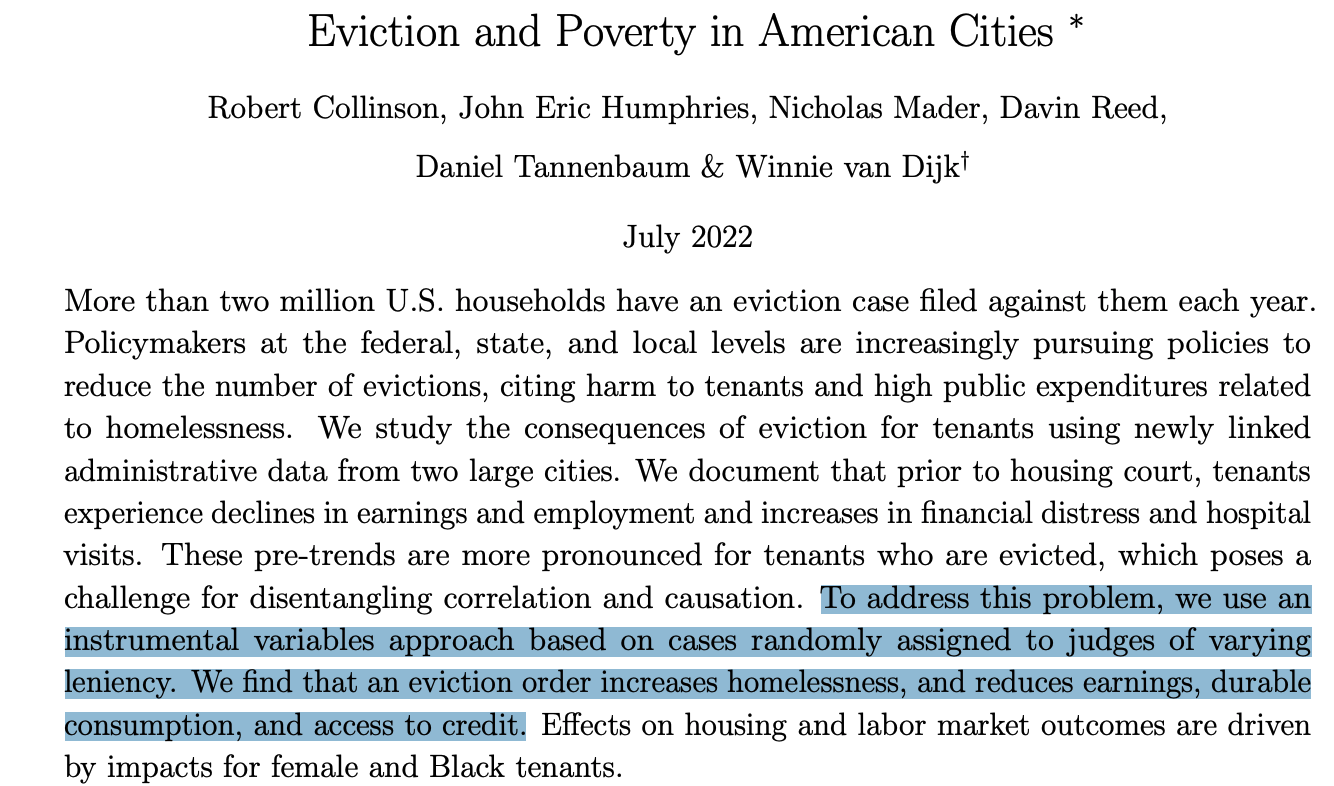
\includegraphics[width= 0.9 \linewidth]{eviction}
\end{frame}

\end{document}


